\section{Benchmark Protocol}
\label{sec:data}

\begin{figure}[!t]
\centering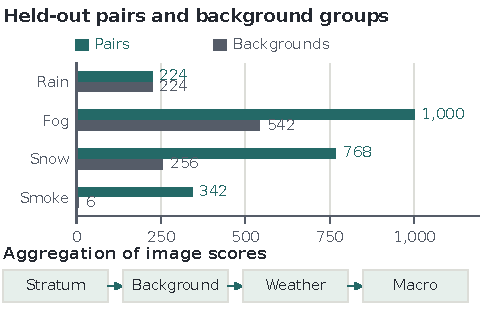
\includegraphics[width=\linewidth]{figures/benchmark_protocol.pdf}
\caption{Test coverage and aggregation. The 342 smoke pairs come from six backgrounds. Image scores are averaged within strata and then across strata, backgrounds, and weather conditions with equal weights at each level.}
\label{fig:benchmark-protocol}
\end{figure}
\paragraph{Paired data.}
The active mixture combines processed real-rain pairs from RealRain-1k-H~\cite{Li_2022_RealRain}, source-generated RESIDE-6K haze as a fog proxy, SnowCityscapes synthetic snow, and surveillance smoke from a repaired SmokeBench~\cite{Jin_2025_SmokeBench} partition. The source datasets supply all weather effects. Table~\ref{tab:data} reports the frozen split, including background groups. Figure~\ref{fig:benchmark-protocol} relates test coverage to the aggregation rule.

\begin{table}[!t]
\centering\small\setlength{\tabcolsep}{4pt}
\caption{Active paired split. Parentheses give background groups, which may contain related observations.}
\label{tab:data}
\begin{tabular}{@{}lrrr@{}}\toprule
\rowcolor{aegishead}
Source & Train & Val. & Test\\\midrule
RealRain-1k-H &773 (755)&112 (112)&224 (224)\\
RESIDE-6K &5,102 (5,061)&897 (893)&1,000 (542)\\
SnowCityscapes &5,382 (1,794)&618 (206)&768 (256)\\
SmokeBench &7,353 (31)&384 (6)&342 (6)\\\midrule
Total pairs &18,610&2,011&2,334\\\bottomrule
\end{tabular}
\end{table}

A decode audit of 52,140 active and reserve files finds zero exact cross-split overlaps or near-target candidates under the specified thumbnail and pHash rule. The repaired split removes the identified smoke-reference overlap. Reserved snow/smoke pairs stay excluded from selection and testing. Sequence independence and alignment remain imperfectly characterized. Supplementary Appendix~A gives the audit thresholds and reserve counts.

\paragraph{Aggregation.}
For per-image RGB PSNR or SSIM $m_i$, let $I_s$ be images in stratum $s$, $S_g$ strata for background $g$, and $G_w$ backgrounds for weather $w$. We report
\begin{equation}
\bar m=\frac14\sum_w\frac1{|G_w|}\sum_{g\in G_w}
\frac1{|S_g|}\sum_{s\in S_g}\frac1{|I_s|}\sum_{i\in I_s}m_i.
\label{eq:metric}
\end{equation}
Strata rank thumbnail input/target differences within each background as a degradation proxy. Equal weighting at each level limits the influence of many variants from a single scene. Evaluation uses native-resolution BF16 forward passes and RGB in $[0,1]$, with MSE floor $10^{-12}$ and uniform $7\times7$ sample-covariance SSIM. Metrics precede 8-bit export. All 14,004 model/image rows support reaggregation. Cluster resampling estimates uncertainty conditional on these checkpoints and test groups.
